\chapter{Tight Splitting and Jointless Tracks}
\label{chap:tight_splitting}

For the purpose of classifying all pseudo-Anosov braids on $D_6$ in the strata $(3;1^6;3)$ and $(2;1^6;3^2)$ which lift to fixed-point-free pseudo-Anosov maps, we utilize the \texttt{autofolder} program to output all standard train track isomorphism classes for these strata. For each of these isomorphism classes, the program provides one standard train track representative; thus, for each of the two strata, we obtain a finite list of standard train tracks (encoded as \texttt{StandardTrainTrack} objects). By Proposition \ref{prop:every_pA_carried_by_standard_track}, every pseudo-Anosov 6-braid $\beta$ in each stratum is carried by one of these standard train tracks.

We can further reduce the number of standard train tracks to consider by invoking a result of Farber, Reinoso, and Wang \sidecite{farber2024fixed}, which states that in most strata, every pseudo-Anosov map is conjugate to one carried by what they term ``jointless'' train tracks. A \emph{joint} on a standard train track is a switch located at a marked monogon with more than one adjacent real edge. To demonstrate this, they developed the notion of an operation called \emph{tight splitting} on standard train tracks. As mentioned previously, there is a more general operation of splitting, due to Penner and Harer \sidecite{penner1992combinatorics}, which can be viewed as the geometric inverse of folding. The tight splitting of Farber-Reinoso-Wang is a specific instance of splitting---precisely the inverse of the elementary folding defined in Chapter \ref{chap:folding_automata}.

Crucially, a tight splitting guarantees that the resultant train track carries the same train track map as the original (up to conjugation by a braid). Using tight splittings, Farber, Reinoso, and Wang show that all joints of a standard train track $\tau$ carrying a train track map $f$ can be removed via a finite sequence of tight splittings. This process produces a jointless train track $\tau'$ that still carries $f$, up to conjugation.

We utilize this strategy to reduce the number of standard train tracks to consider from the \texttt{autofolder} output. We demonstrate that for the majority of standard train tracks in the list, a finite sequence of tight splittings leads to a select subset of tracks. Consequently, up to conjugation, any pseudo-Anosov braid is carried by this smaller set of train tracks. Furthermore, for the purpose of identifying the knot monodromy $h$ associated with the braid via the Birman-Hilden correspondence, we may consider braids up to mirroring. This allows for a further reduction by identifying pairs of standard jointless train tracks that are mirror images of one another and selecting a single representative from each pair.

\paragraph{Notation reminder.} Throughout this chapter we fix a pseudo-Anosov braid $\beta \in \mathrm{Mod}(D_n)$ with geometric data $(\beta, \phi_\beta, \tau, f_\beta)$, in the sense of Chapter \ref{chap:train tracks}: $\beta$ is the braid (mapping class), $\phi_\beta \colon D_n \to D_n$ is its pseudo-Anosov representative, $\tau$ is a standard train track carrying $\phi_\beta$, and $f_\beta \colon \tau \to \tau$ is the induced train-track map. This is the data on which all of the splitting operations below act. The associated lift $(\Phi, \phi_\Phi)$ to $\Sigma_2^2$ via the Birman-Hilden correspondence (Chapter \ref{chap:preliminaries}) is what ultimately matters for the knot-detection argument, but the train-track operations themselves take place entirely on the disk level.

\section{Splitting Standard Train Tracks}
\label{sec:splitting-standard}

The goal of tight splitting is to reverse the elementary folding process (Definition \ref{def:elementary_folding_map}) in a manner that preserves the property of carrying a specific pseudo-Anosov map. To achieve this, we first rigorously define the local coordinates and orientation at a switch.

\subsection{Branches at a switch}
\label{subsec:local-coordinates}

To formalize the splitting operation, we require precise notation for the local geometry of the train track $\tau \subset D_n$ near a switch.

\begin{definition}[Incoming Real Edges]
Let $v$ be a switch of $\tau$. We adopt the convention that real edges incident to $v$ are oriented \textbf{towards} $v$. We denote the set of incoming real edges at $v$ by $R(v)$. Since $\tau$ is standardly embedded in the oriented disk $D_n$, the set $R(v)$ admits a natural linear ordering induced by the counter-clockwise orientation of the tangent space at $v$. This linear ordering is a subset of the ordering described in the definition of the combinatorial structure $\mathcal{C}(\tau) = (G,\mathcal{O},\ell)$ of $\tau$, where $\mathcal{O}$ records the cyclic ordering at each switch (both infinitesimal and real).
\end{definition}

\begin{definition}[Left and Right Edges]
Let $v$ be a switch with $R(v) \neq \emptyset$.
\begin{enumerate}
    \item We define $l(v) \in R(v)$ to be the minimal element of $R(v)$ with respect to the local ordering. We refer to $l(v)$ as the \textbf{leftmost incoming edge} at $v$.
    \item We define $r(v) \in R(v)$ to be the maximal element of $R(v)$. We refer to $r(v)$ as the \textbf{rightmost incoming edge} at $v$.
\end{enumerate}
\end{definition}

\begin{definition}[Source Switches and Composite Notation]
For the distinguished edges $l(v)$ and $r(v)$, we denote their source vertices as follows:
\begin{itemize}
    \item Let $v_l$ denote the source vertex of $l(v)$ (i.e., $l(v)$ is directed from $v_l$ to $v$).
    \item Let $v_r$ denote the source vertex of $r(v)$ (i.e., $r(v)$ is directed from $v_r$ to $v$).
\end{itemize}
Consequently, the notation $r(v_l)$ refers to the rightmost incoming edge at the switch $v_l$, and $l(v_r)$ refers to the leftmost incoming edge at the switch $v_r$.
\end{definition}

\subsection{Tight Splitting and Stability}

With these local coordinates established, we define the tight splitting operation.

\begin{definition}[Tight Splitting]
\label{def:tight-splitting}
Let $\tau \hookrightarrow D_n$ be a standardly embedded train track, let $v$ be a switch of $\tau$, and fix a train track map $f \colon \tau \to \tau$.
We say that $v$ \textbf{splits tightly to the left} (or \textbf{\textit{l}-splits}) if for every real edge $x \subseteq \tau$, the following conditions hold regarding the image path $f(x)$:
\begin{enumerate}
    \item Whenever the edge $l(v)$ appears in the train path $f(x)$, it is immediately followed by the edge $r(v_l)$ (traversed against its orientation).
    \item Whenever the edge $l(v)$ appears in the train path $f(x)$, it is immediately preceded by the edge $r(v_l)$ (traversed along its orientation).
\end{enumerate}
Similarly, we say that $v$ \textbf{splits tightly to the right} (or \textbf{\textit{r}-splits}) if the analogous conditions hold with the roles of ``left'' and ``right'' reversed (i.e., replacing $l(v)$ with $r(v)$ and $r(v_l)$ with $l(v_r)$).
\end{definition}

If a switch $v$ splits tightly, we construct a new train track $\tau_v^l$ (in the case of an $l$-split) which maps to $\tau$ via an elementary folding map. We use the notation $\tau_v^t$ to refer generically to the result of either an $l$-split or an $r$-split.

\paragraph{Construction of the Split Track $\tau_v^l$.}
Suppose $v$ $l$-splits. We define $\tau_v^l$ to be the standardly embedded train track obtained from $\tau$ by deleting the edge $l(v)$ and replacing it with a new real edge $\alpha$ satisfying the following conditions:
\begin{enumerate}
    \item As a directed edge, the source and target of $\alpha$ are given by $\alpha(0) = l(v)(0)$ and $\alpha(1) = r(v_l)(1)$.
    \item The edge $\alpha$ forms a bigon (a two-cusped disk) with the train path $l(v) \cdot \overline{r(v_l)}$, and there is an isotopy relative to the punctures of $D_n$ such that $\alpha$ lies transverse to the measured foliation.
\end{enumerate}
The construction of $\tau_v^r$ (when $v$ $r$-splits) is symmetric.

This construction is the precise geometric inverse of the elementary folding operation described in Chapter \ref{chap:folding_automata}. Specifically, the transformation $\tau \to \tau_v^l$ corresponds to the inverse of the elementary folding map
\[
p\colon \tau_v^l \to \tau,
\]
where the folding operation maps the edge $\alpha$ onto $l(v)$ and $r(v_l)$ (effectively folding the ``new'' branch back into the ``old'' branch).

\begin{figure}[ht]
    \centering
    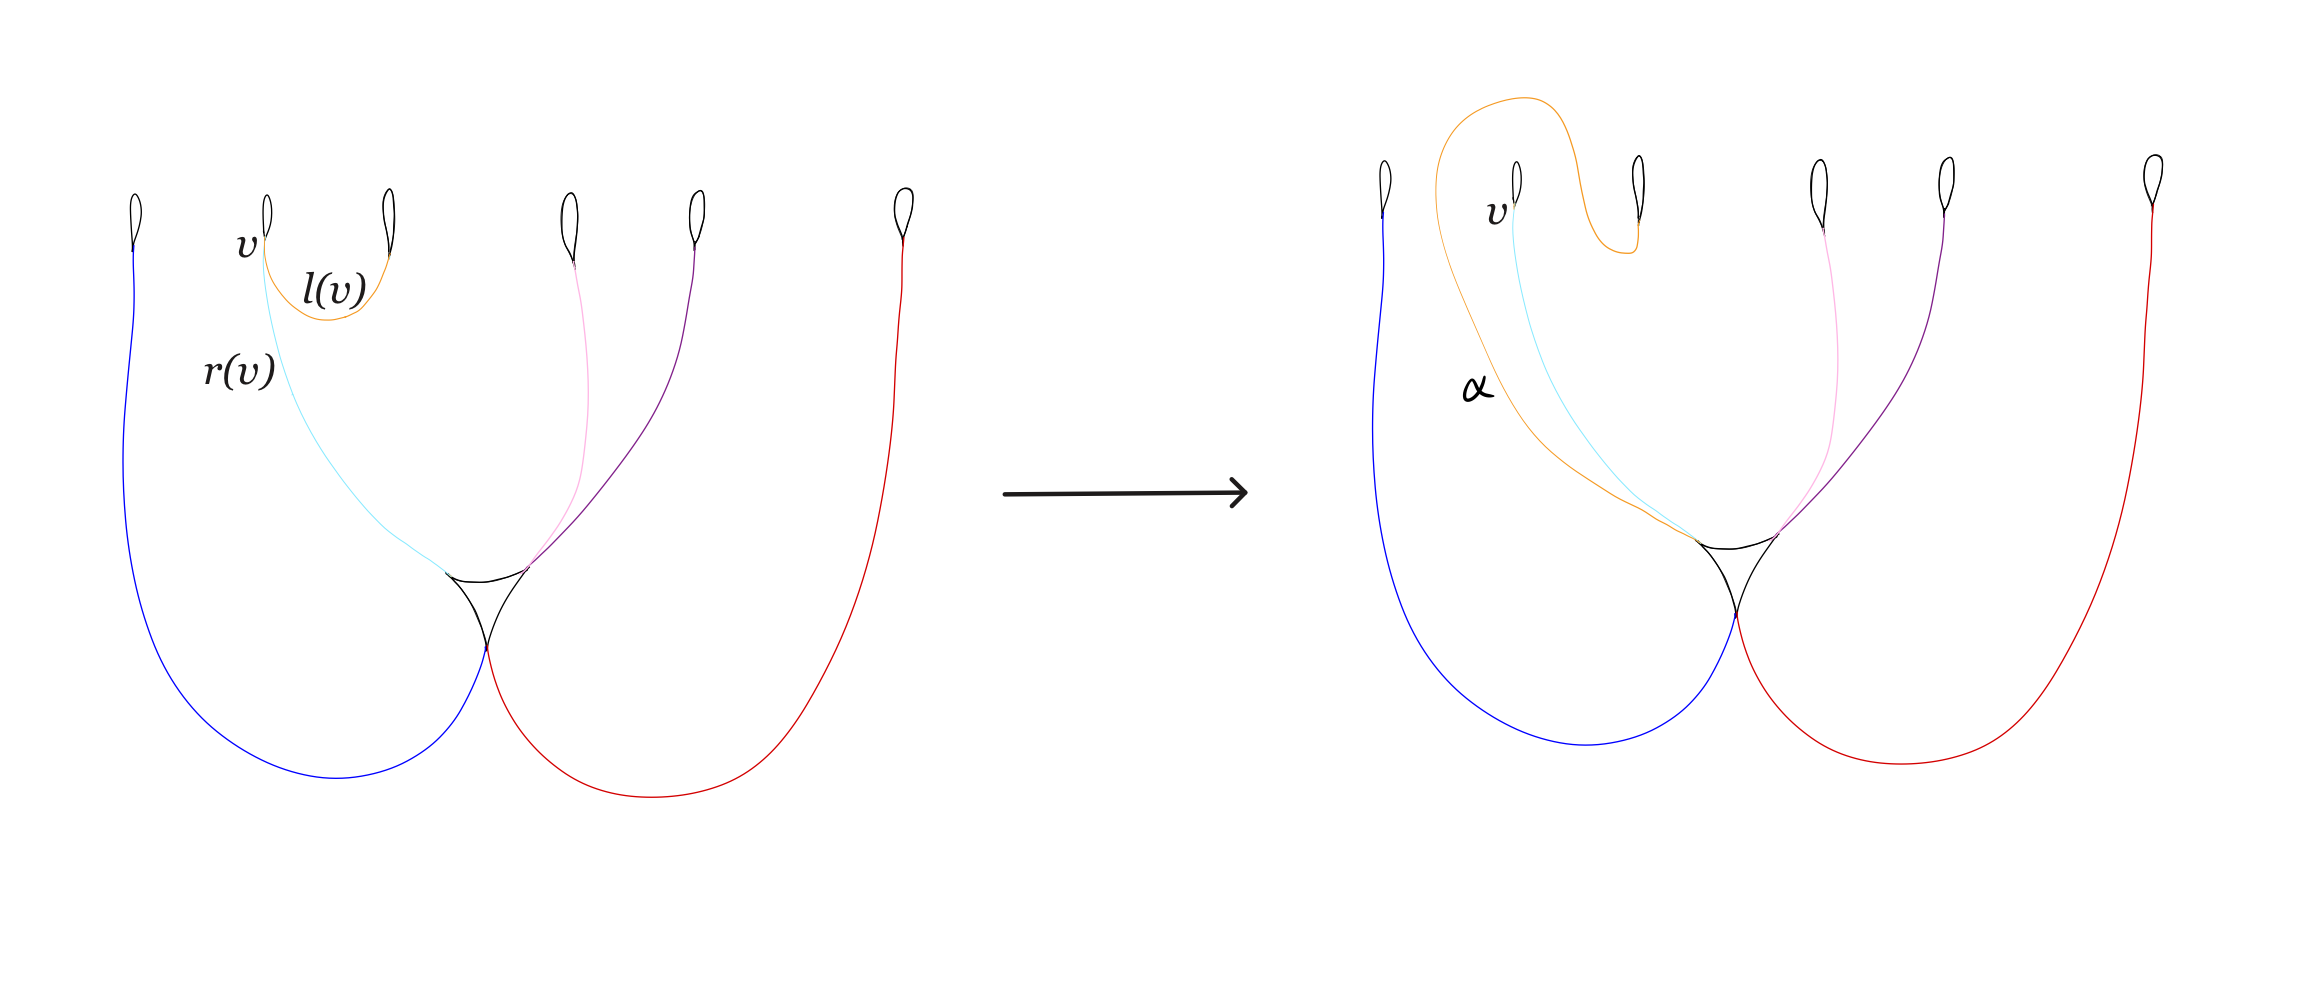
\includegraphics[width=\linewidth]{figures/splitting.png}
    \caption{An $l$-split at the vertex $v$. Notice this is the exact inverse of the folding operation $p$ of Figure \ref{fig:folding}.}
    \label{fig:splitting}
\end{figure}

\begin{remark}
    While the geometric construction of the split track $\tau_v^t$ can be performed at any switch $v$ with sufficient valence, the definition of a \emph{tight} splitting requires the existence of a compatible train track map $f \colon \tau \to \tau$ that respects the local folding structure.
\end{remark}

\subsection{Dynamics and the Transition Matrix}

The primary utility of tight splitting is encapsulated in the following results, which ensure that the dynamic properties of the map (such as the dilatation) are preserved.

\begin{prop}[{\cite[Proposition~6.1.7]{reinoso2024pseudo}}]
\label{prop:carrying_preserved_under_split}
    Retain the notation $(\beta, \phi_\beta, \tau, f_\beta)$ from above, with $\tau$ a standard train track carrying the pseudo-Anosov $\phi_\beta$. Suppose $\tau$ splits tightly to the left at a switch $v$ to produce the train track $\tau_v^l$. Then, up to conjugacy by a braid, $\phi_\beta$ is carried by $\tau_v^l$. We denote the associated train track map on $\tau_v^l$ by
    \[
    f_{\beta, v}^{l} \colon \tau_{v}^{l} \to \tau_{v}^{l}.
    \]
    An analogous result holds if $\tau$ splits tightly to the right.
\end{prop}

In the language of folding automata, a tight splitting implies that traversing a cycle representing a pseudo-Anosov map corresponds to a reverse traversal of elementary foldings. The transition matrices of the split and original tracks are related by conjugation via the folding matrix.

\begin{prop}[{\cite[Proposition~6.1.8]{reinoso2024pseudo}}]
\label{prop:transition_matrix_split}
Retain the notation of Proposition \ref{prop:carrying_preserved_under_split}. Suppose that $\tau$ \textit{l}-splits at $v$, and let $M$ and $M_{v}$ be the transition matrices of $f_\beta \colon \tau \to \tau$ and $f_{\beta, v}^{l} \colon \tau_{v}^{l} \to \tau_{v}^{l}$ respectively. Then
\[
M_v = P^{-1}MP,
\]
where $P$ is the transition matrix of the elementary folding map
\[
p \colon \tau_{v}^{l} \to \tau
\]
associated with the inverse of the tight splitting. Concretely, if $l(v)$ is the $j$th real edge of $\tau$ and $r(v_l)$ is the $i$th real edge, then
\[
P = I_n + D_{i,j},
\]
where $D_{i,j}$ is the elementary matrix with a $1$ in entry $(i,j)$ and zeros elsewhere.
\end{prop}

The tight splitting condition imposes a strict inequality on the invariant measure (the weights) of the branches involved.

\begin{prop}[{\cite[Corollary~6.1.9]{reinoso2024pseudo}}]
\label{prop:weight_inequality}
Retain the notation $(\beta, \phi_\beta, \tau, f_\beta)$ for a pseudo-Anosov braid carried by a standardly embedded train track. Let $M$ be the transition matrix for $f_\beta \colon \tau \to \tau$, and let $\lambda$ be the dilatation of $f_\beta$. Fix a positive right $\lambda$-eigenvector $\mu$ of $M$ representing the transverse measure. If $v$ \textit{l}-splits, then $\mu_{v}=P^{-1}\mu$ is a positive right $\lambda$-eigenvector of $M_{v}$. Consequently, the weights satisfy the inequality:
\[
\mu(l(v)) < \mu(r(v_l)).
\]
Similarly, if $v$ \textit{r}-splits, then $\mu(r(v)) < \mu(l(v_r))$.
\end{prop}

The utility of Proposition \ref{prop:weight_inequality} becomes apparent when analyzing a tight splitting at a switch where the resulting track is isomorphic to the original. This situation arises, in particular, at loop switches (switches at a marked monogon), but it also occurs at switches incident to higher-order infinitesimal polygons in the splitting diagrams of Section \ref{sec:switch-rigidity}.

\begin{corollary}
\label{cor:weight_reduction}
    Suppose a switch $v$ of a standard train track $\tau$ carrying a pseudo-Anosov $\phi_\beta$ \textit{l}-splits, such that the resulting train track $\tau_v^l$ is isomorphic to $\tau$. Let $\varphi \colon \tau_v^l \to \tau$ be the isomorphism (given by a braid). Then the weight of the branch corresponding to $r(v_l)$ strictly decreases. That is, if $\mu$ is the invariant measure on $\tau$ and $\mu_v$ is the measure on $\tau_v^l$, then:
    \[
    \mu_v(r(v_l)_{new}) < \mu(r(v_l)_{old}).
    \]
    The analogous statement holds for $r$-splits, with $r(v_l)$ replaced by $l(v_r)$.
\end{corollary}

\begin{proof}
    Let $p \colon \tau_v^l \to \tau$ be the elementary folding map associated with the tight splitting. This map identifies the new edge $\alpha$ with $l(v)$ and the new branch $r(v_l)_{new}$ with $r(v_l)_{old}$. The relationship between the transverse measures is given by the pullback of $p$, which satisfies the additivity equation:
    \[
    \mu(r(v_l)_{old}) = \mu_v(r(v_l)_{new}) + \mu_v(\alpha).
    \]
    By Proposition \ref{prop:weight_inequality}, the eigenvector $\mu_v$ is well-defined and positive. Furthermore, the proposition establishes that for the splitting to be valid (tight), the weights must satisfy the strict inequality $\mu(l(v)) < \mu(r(v_l)_{old})$.

    Since the splitting operation assigns the weight of the removed edge $l(v)$ to the new edge $\alpha$ (i.e., $\mu_v(\alpha) = \mu(l(v))$), and since $\mu$ is a positive eigenvector for a pseudo-Anosov map, we have $\mu_v(\alpha) > 0$.

    Substituting this back into the additivity equation yields:
    \[
    \mu_v(r(v_l)_{new}) = \mu(r(v_l)_{old}) - \mu(l(v)).
    \]
    Because $\mu(l(v))$ is strictly positive, it follows immediately that:
    \[
    \mu_v(r(v_l)_{new}) < \mu(r(v_l)_{old}).
    \]
    Thus, under the isomorphism $\varphi$ which maps the edge $r(v_l)_{new}$ back to $r(v_l)_{old}$, the weight associated with this edge orbit strictly decreases.
\end{proof}

\begin{corollary}
\label{cor:termination}
    Let $\tau$ be a standard train track and $f_\beta \colon \tau \to \tau$ a train track map induced by a pseudo-Anosov $\phi_\beta$. Suppose
    \[
    \tau = \tau_0 \to \tau_1 \to \tau_2 \to \cdots
    \]
    is a sequence of tight splittings of $\tau$, each step being either an $l$-split or an $r$-split. Then $\tau$ cannot reappear in this sequence infinitely many times; that is, the set $\{ i \ge 0 : \tau_i \cong \tau \}$ is finite. More generally, no isomorphism class of standard tracks can be visited infinitely often in any sequence of tight splittings.
\end{corollary}
\begin{proof}
    Suppose, for contradiction, that there are infinitely many indices $i_1 < i_2 < \cdots$ with $\tau_{i_k} \cong \tau$. By Proposition \ref{prop:weight_inequality} and the additivity calculation in the proof of Corollary \ref{cor:weight_reduction}, each tight splitting strictly decreases the transverse weight on at least one real edge (the $r(v_l)$ or $l(v_r)$ edge of the split switch), while leaving all other weights non-increased. Tracking the maximum weight on the edge corresponding to $r(v_l)$ (or $l(v_r)$) along the subsequence $\{\tau_{i_k}\}$ under the iso-class identification with $\tau$, we obtain a strictly decreasing sequence of positive real numbers, hence converging to $0$. But the transverse measure of a pseudo-Anosov is everywhere strictly positive on real edges, a contradiction. The same argument applies to any other isomorphism class visited infinitely often: cycles of splits returning to a fixed iso class strictly decrease some weight, and that weight cannot converge to $0$ while staying positive.
\end{proof}

\begin{theorem}[Termination of Tight Splitting]
\label{thm:splitting_termination}
    Let $(\beta, \phi_\beta, \tau, f_\beta)$ be the geometric data of a pseudo-Anosov braid carried by a standard train track $\tau$. There exists no infinite sequence of tight splittings starting from $\tau$.
\end{theorem}

\begin{proof}
    Suppose, for contradiction, that there exists an infinite sequence of tight splittings
    \[
    \tau = \tau_0 \to \tau_1 \to \tau_2 \to \cdots
    \]
    starting from $\tau$. By Theorem~\ref{thm:autofolder_main}, the set of isomorphism classes of standard train tracks in a fixed stratum on $D_n$ is finite. Since each $\tau_i$ lies in the same stratum as $\tau$ (tight splitting preserves singularity data), the pigeonhole principle forces at least one isomorphism class $[\tau^\ast]$ to be visited infinitely often along the sequence. But this contradicts Corollary \ref{cor:termination}, which forbids any isomorphism class from being visited infinitely often in any sequence of tight splittings.

    Thus, no infinite sequence of tight splittings starting from $\tau$ exists.
\end{proof}

\section{Switch Rigidity and Existence of Splits}
\label{sec:switch-rigidity}

The following proposition of Reinoso \cite[Corollary~6.2.9]{reinoso2024pseudo}, building on the broader work of Farber-Reinoso-Wang \sidecite{farber2024fixed}, is instrumental in their proof that every train track map is carried by a jointless train track, essentially showing that any joint at a loop switch can be split.

\begin{prop}[Existence of Splittable Switches, {\cite[Corollary~6.2.9]{reinoso2024pseudo}}]
\label{prop:reinoso_6.2.9_splittable}
Let $n_k$ denote the maximal real valence of a switch at an infinitesimal $k$-gon of $\tau$, where $k \ge 1$. If $n_k > 1$, then there exists a switch of valence $n_k$ at such a $k$-gon which $l$-splits or $r$-splits. In particular, if the train track has any switch with valence greater than 1, there exists at least one switch that $l$-splits or $r$-splits.
\end{prop}

For our purposes, the result provides a sufficient condition to guarantee a switch can be split. This provides the inductive step for our reduction procedure: at every $k$-gon, a unique switch of maximal valence can always be split.

\subsection*{Splitting Diagram}

We now illustrate how Proposition \ref{prop:reinoso_6.2.9_splittable} (existence of a splittable switch) and Corollary \ref{cor:termination} (no isomorphism class is visited infinitely often) combine in practice to constrain which train tracks must carry a given pseudo-Anosov map. The following diagram traces all possible tight splittings emanating from a particular standard jointless train track labeled (1.) in the stratum $(3; 1^6; 3)$. The upshot is that any train track map carried by (1.) must, after a finite sequence of tight splittings, be carried by one of two specific terminal tracks --- labeled (12.) and (0.) in the diagram.

\begin{figure}[htbp]
    \centering
    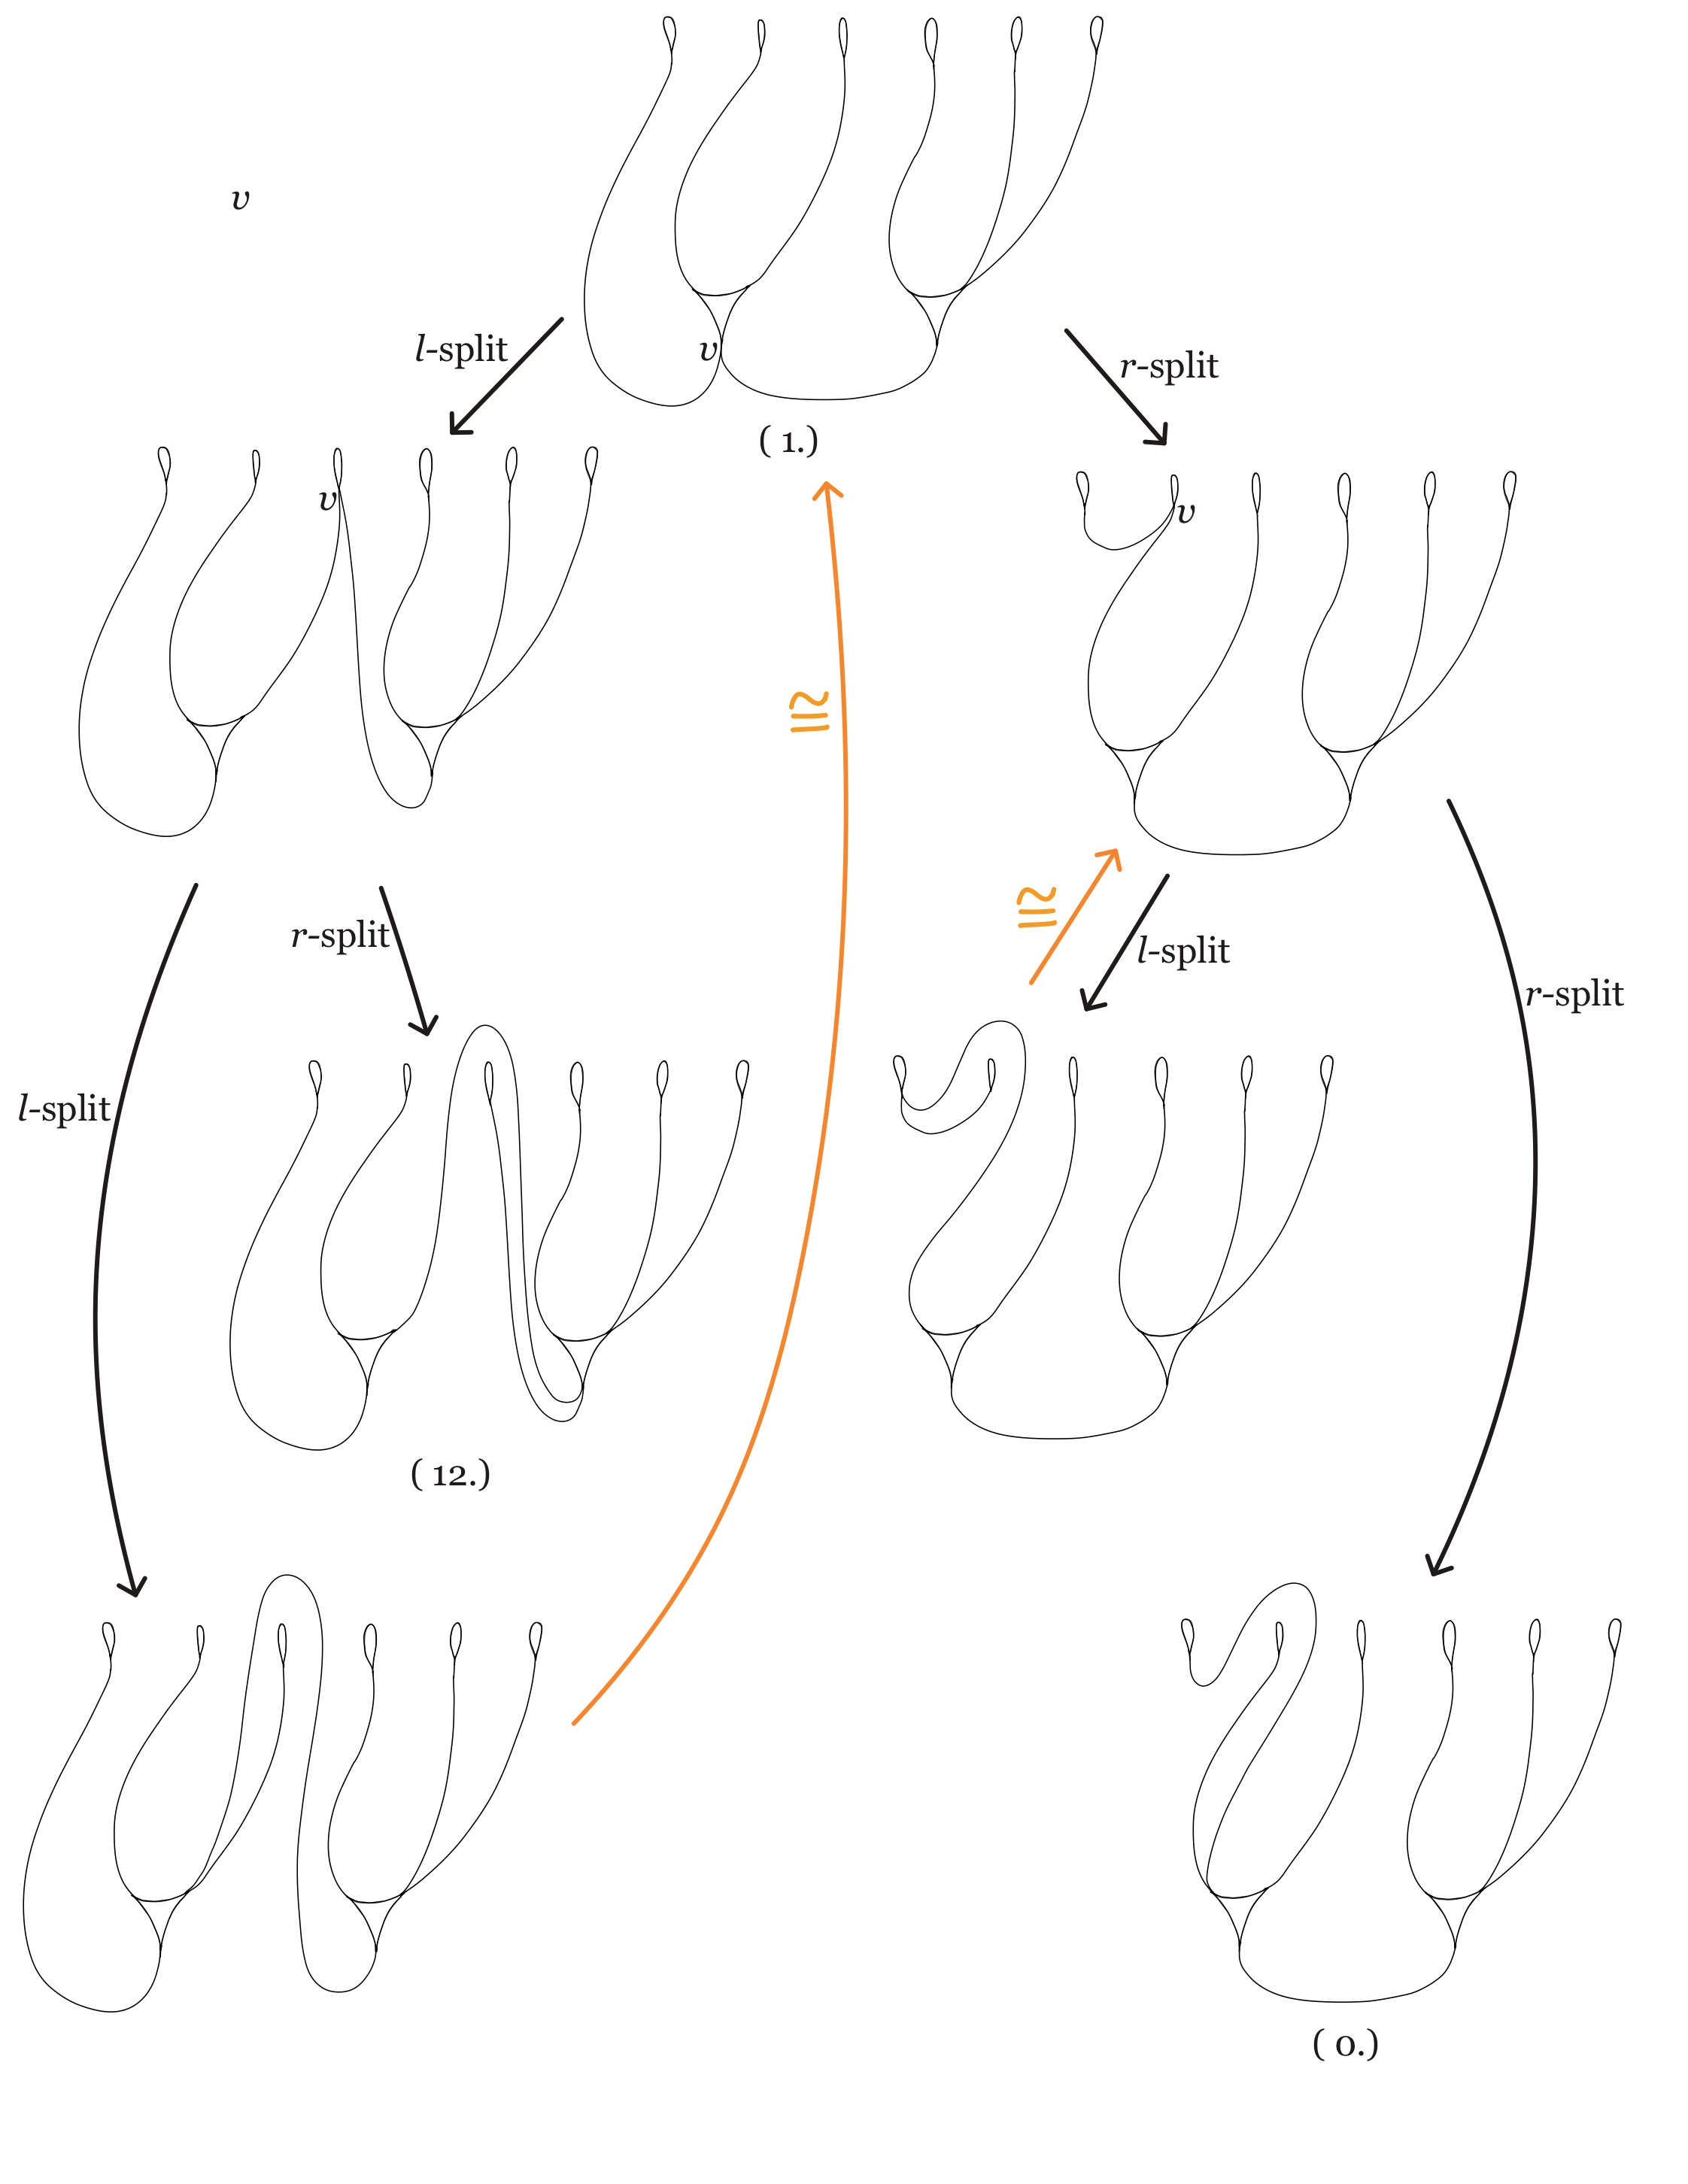
\includegraphics[width=\textwidth]{figures_splitting/1 Splitting-2.jpg}
    \sidecaption{This splitting diagram shows that any train track map carried by train track (1.) must also be carried by train track (12.) or (0.), up to the action of a braid.}
    \label{fig:split_diagram_example}
\end{figure}

Figure \ref{fig:split_diagram_example} shows a sequence of splittings starting from the standard jointless train track labeled (1.). We implicitly assume that there is a train track map carried by this train track (1.). Consider the triangle, i.e., the $3$-gon, on the left of this train track. The maximal real valence of a switch at this infinitesimal $3$-gon is 2. Specifically, the switch $v$ is the unique switch of maximal real valence.

By Proposition \ref{prop:reinoso_6.2.9_splittable}, $v$ must either $l$-split or $r$-split. If it $l$-splits, we traverse to the left-hand side of the diagram to a standard train track with a joint labeled $v$ again. Invoking Proposition \ref{prop:reinoso_6.2.9_splittable} once more, this train track either $l$-splits or $r$-splits. For the $r$-split case, we arrive at a train track labeled (12.). For the $l$-split case, we arrive at a train track at the bottom left of the diagram, which is isomorphic to the original train track (1.).

Going back to the initial splitting of (1.), the $r$-split scenario yields a train track which $l$-splits to itself, and $r$-splits to the train track (0.).

In this diagram, at each bifurcation, Proposition \ref{prop:reinoso_6.2.9_splittable} guarantees that at least one of an $l$-split or an $r$-split occurs, but not necessarily both. On the other hand, Corollary \ref{cor:termination} disallows infinite repeating sequences of splittings of a train track back to itself (or a train track isomorphic to itself); in other words, any sequence of tight splittings on the diagram must eventually result in train track (12.) or train track (0.). Otherwise, such a sequence would include infinite revisits of the same train track. Therefore, Figure \ref{fig:split_diagram_example} demonstrates that given any train track map $f$ carried by train track (1.), $f$ is also carried by train track (12.) or (0.), up to an action by a braid.

We call a diagram such as Figure \ref{fig:split_diagram_example} a \textbf{splitting diagram}. In our analysis of the non-orientable strata $(3;1^6;3)$ and $(2;1^6;3^2)$, we aim to classify all train track maps in these strata lifting to fixed-point-free pseudo-Anosov maps. As will be shown, we make use of these splitting diagrams to drastically reduce the number of candidate train tracks to consider in our final topological analysis.

\section{Conclusion}

In this chapter, we addressed the proliferation of redundant states inherent in the unrestricted folding automaton. Because the \texttt{autofolder} algorithm exhaustively executes every valid elementary fold at every available cusp, it generates a state space that contains many valid but topologically redundant standard train tracks --- specifically those burdened by joints. By deploying the tight splitting operation, we established a rigorous reduction procedure to mathematically prune this state space for our non-orientable strata. The first stage of this reduction, the elimination of joints at loop switches (i.e., switches incident to a marked monogon), was established by Reinoso in his thesis \sidecite{reinoso2024pseudo}; we then go further, applying tight splittings at non-loop switches (e.g., the switches of maximal real valence on infinitesimal triangles) to prune the resulting list of jointless tracks even more.

As guaranteed by the termination of tight splitting (Theorem \ref{thm:splitting_termination}), this reduction process is finite. In Chapter \ref{chap:stratatraintrackanalysis}, we will execute this procedure, utilizing the splitting diagrams introduced above to systematically collapse the raw output of our \texttt{autofolder} algorithm.

Through this reduction, we will demonstrate that any pseudo-Anosov mapping class belonging to the strata $(3;1^6;3)$ or $(2;1^6;3^2)$ on $D_6$ must, up to braid conjugation and mirroring, be carried by a small, manageable number of jointless standard train tracks. Once this finite collection is established, we will explicitly enumerate, by hand, all possible train track maps carried by each such track, and apply the Trace Lemma (Lemma \ref{lem:trace_lemma}) and its jointless-monogon corollary (Corollary \ref{cor:trace_lemma_jointless}) directly to each candidate train-track map to rule out the existence of a fixed-point-free lift, thereby completing the proof of our main detection theorem.